\documentclass{article}
\usepackage{tikz}
\usepackage{amsmath}
\usepackage{amssymb}

% Define notation for integer interval
\newcommand{\intint}[1]{\llbracket #1 \rrbracket}

\begin{document}

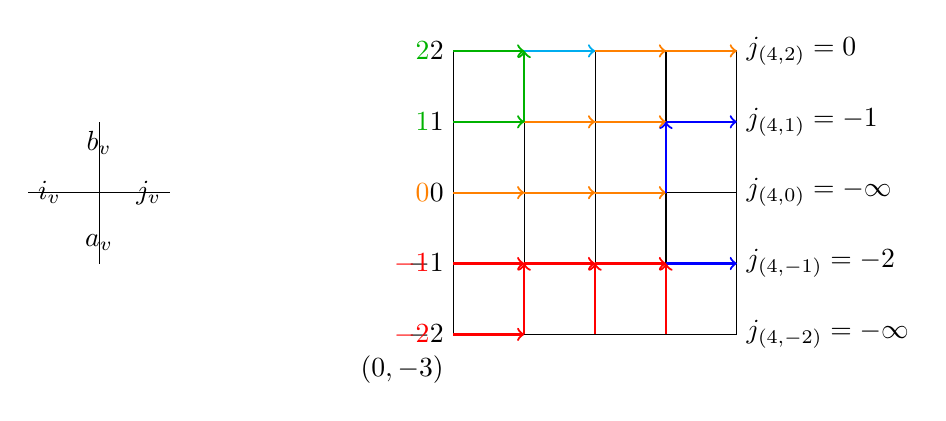
\begin{tikzpicture}[scale=0.9]
    % Left diagram - vertex labels
    \begin{scope}[shift={(-2.5,0)}]
        % Draw the cross
        \draw (-1,0) -- (1,0);
        \draw (0,-1) -- (0,1);
        
        % Add labels
        \node at (-0.7,0) {$i_v$};
        \node at (0.7,0) {$j_v$};
        \node at (0,0.7) {$b_v$};
        \node at (0,-0.7) {$a_v$};
    \end{scope}
    
    % Right diagram - six-vertex model
    \begin{scope}[shift={(2.5,0)}]
        % Draw the grid
        \draw (0,-2) grid (4,2);
        
        % Add y-axis labels
        \node[left] at (0,2) {$2$};
        \node[left] at (0,1) {$1$};
        \node[left] at (0,0) {$0$};
        \node[left] at (0,-1) {$-1$};
        \node[left] at (0,-2) {$-2$};
        \node[left] at (0,-2.5) {$(0,-3)$};
        
        % Add arrows with colors
        % Row 2 (y=2)
        \draw[->, green!70!black, thick] (0,2) -- (1,2);
        \draw[->, cyan, thick] (1,2) -- (2,2);
        \draw[->, orange, thick] (2,2) -- (3,2);
        \draw[->, orange, thick] (3,2) -- (4,2);
        
        % Row 1 (y=1)
        \draw[->, green!70!black, thick] (0,1) -- (1,1);
        \draw[->, orange, thick] (1,1) -- (2,1);
        \draw[->, orange, thick] (2,1) -- (3,1);
        \draw[->, blue, thick] (3,1) -- (4,1);
        
        % Row 0 (y=0)
        \draw[->, orange, thick] (0,0) -- (1,0);
        \draw[->, orange, thick] (1,0) -- (2,0);
        \draw[->, orange, thick] (2,0) -- (3,0);
        
        % Row -1 (y=-1)
        \draw[->, red, thick] (0,-1) -- (1,-1);
        \draw[->, red, thick] (1,-1) -- (2,-1);
        \draw[->, red, thick] (2,-1) -- (3,-1);
        \draw[->, blue, thick] (3,-1) -- (4,-1);
        
        % Row -2 (y=-2)
        \draw[->, red, thick] (0,-2) -- (1,-2);
        
        % Vertical arrows
        \draw[->, green!70!black, thick] (1,1) -- (1,2);
        \draw[->, blue, thick] (3,0) -- (3,1);
        \draw[->, red, thick] (1,-2) -- (1,-1);
        \draw[->, red, thick] (2,-2) -- (2,-1);
        \draw[->, red, thick] (3,-2) -- (3,-1);
        
        % Color labels on left boundary
        \node[green!70!black, left] at (-0.2,2) {$2$};
        \node[green!70!black, left] at (-0.2,1) {$1$};
        \node[orange, left] at (-0.2,0) {$0$};
        \node[red, left] at (-0.2,-1) {$-1$};
        \node[red, left] at (-0.2,-2) {$-2$};
        
        % Add j function values on right
        \node[right] at (4,2) {$j_{(4,2)} = 0$};
        \node[right] at (4,1) {$j_{(4,1)} = -1$};
        \node[right] at (4,0) {$j_{(4,0)} = -\infty$};
        \node[right] at (4,-1) {$j_{(4,-1)} = -2$};
        \node[right] at (4,-2) {$j_{(4,-2)} = -\infty$};
    \end{scope}
\end{tikzpicture}

\end{document}